\documentclass[10pt,a4paper]{article}
\usepackage[utf8]{inputenc}
\usepackage{grffile}
\usepackage{graphicx}
\usepackage{lmodern}
\usepackage{fourier}
\author{Austin Vern Songer}
\begin{document}
\tableofcontents
%--------------------------------------------------------------------------------------------------
\newpage
\part{What Is A Virtual Private Network (VPN)}
%--------------------------------------------------------------------------------------------------
A virtual private network (VPN) is an extension of an enterprise's private intranet
across a public network such as the Internet, creating a secure private
connection, essentially through a private tunnel. VPNs securely convey
information across the Internet connecting remote users, branch offices, and
business partners into an extended corporate network

\section{It Is Virtual}
This means that the physical infrastructure of the network has to be
transparent to any VPN connection. In most cases it also means that the
physical network is not owned by the user of a VPN but is a public network
shared with many other users. To facilitate the necessary transparency to the
upper layers, protocol tunneling techniques are used. To overcome the
implications of not owning the physical network, service level agreements with
network providers should be established to provide, in the best possible way,
the performance and availability requirements needed by the VPN.



\section{It Is Private}
The term “private” in the VPN context refers to the privacy of the traffic that is
to flow over the VPN. As mentioned before, VPN traffic often flows over public
networks (hence the confusion with the word “private”) and therefore,
precautions must be met to provide the necessary security that is required for
any particular traffic profile that is to flow over a VPN connection. Those
security requirements include:

\begin{itemize}
\item Data encryption
\item Data origin authentication
\item Secure generation and timely refresh of cryptographic keys needed for
encryption and authentication
\item Protection against replay of packets and address spoofing
\end{itemize}



\section{It Is A Network}

Even though not physically existent, a VPN must effectively be perceived and
treated as an extension to a company’s network infrastructure. This means
that it must be made available to the rest of the network, to all or a specified 
subset of its devices and applications, by regular means of topology such as routing and addressing.


%--------------------------------------------------------------------------------------------------
\newpage
\part{Security Considerations}
%--------------------------------------------------------------------------------------------------
\paragraph*{The use of VPNs raises several security concerns beyond those that were
present in traditional corporate networks. A typical end-to-end data path might
contain:}


\begin{itemize}
\item Several machines not under control of the corporation (for example, the ISP
access box in a dial-in segment and the routers within the Internet).
\item A security gateway (firewall or router) that is located at the boundary between
an internal segment and an external segment.
\item An internal segment (intranet) that contains hosts and routers. Some could be
malicious, and some will carry a mix of intracompany and intercompany traffic.
\item An external segment (Internet) that carries traffic not only from your
company's network but also from other sources.
\end{itemize}

\paragraph*{In this environment, there are many opportunities to eavesdrop,
to change a datagram's contents, to mount denial-of-service attacks, or to alter a
datagram's destination address.}


\section{A typical end-to-end path}
To understand the issues with VPN end-to-end security, we look at the elements
along an end-to-end path. While not all the elements may appear in a given path,
some of them will appear in every VPN configuration. 
\\
\\
End-to-end traffic will
usually flow over a mix of three basic segments: a dial-in segment, an external
segment (Internet), and an internal segment (intranet).
\\
\\
A path might include a first-hop dial-in connection to an
Internet service provider (ISP), who in turn uses the backbone public Internet to
carry the user's traffic back to a gateway at the perimeter of the corporate
network. 
\\
\\
Then, the traffic eventually flows within an intranet to its ultimate
destination. Intercompany communication can create
a path that includes two separate intranets (for example, company A's and
company B's).
\\
\\
\subsection{Dial-in segment}
In today's environment, remote access has become a
necessity. Both work-at-home and on-the-road employees want convenient
and secure dial-in access to their company's networks; and sometimes they
even need to communicate with hosts located inside another company's
network. 
\\
\\
We refer to both work-at-home and on-the-road users as remote
users. This segment extends from a remote user's machine to an access box
provided by the ISP. The protocols and procedures used on this link are
specified by the Internet service provider. Today, most ISPs support the
Point-to-Point Protocol (PPP) suite of protocols on this segment.
\\
\\
\subsection{External Network (Internet)}
The Internet is not owned or operated by any
single entity but is a collection of distinct routing domains, each operated by a
different authority. The unifying factor is the standardized IP communications
protocols defined by the Internet Engineering Task Force (IETF).
\\
\\
The Internet
Protocol (IP) suite of protocols will route data traffic at the network layer over a
path that may span several ISPs' routing domains. Since IP is a connectionless technology, each user datagram could potentially follow a
different path. And in fact, traffic from several different companies could all
flow simultaneously through a given backbone router in the Internet. 
\\
\\
For
example, a datagram that originated in company A's intranet and a datagram
that originated in company B's intranet could both flow through a common
router located somewhere in the Internet. A company's traffic on the Internet
can no longer be considered to be isolated from the outside world, as it would
have been on a dedicated private network, since flows from different VPNs will
be intermixed on the Internet backbone.
\\
\\
\subsection{Internal network (Intranet)}
This segment appears at an endpoint of the
communications path. It is under the control of the corporation, which typically
operates and manages it. 
\\
\\
Traditionally, almost all traffic flowing within a
corporate network was generated by the corporation's employees; very little
traffic entered or exited the corporate network; and the protocols in the
intranet were proprietary.

\subsection{Four Classes Of Machines That Occur Along The Path}
\begin{itemize}
\item Remote hosts (dial-up)
\item Fixed hosts (sources and destinations, or clients and servers)
\item ISP access box
\item Security gateways (firewalls and/or routers)
\end{itemize}
\\
\\
Protocols in these machines are used to provide address assignment, tunneling,
and IP security. Viable security solutions can be constructed by deploying IP
security in some combination of remote hosts, firewalls, routers, and fixed hosts.
\\
\\
But since each company should be responsible for its own security, there is no
requirement for the ISP boxes or the routers in the Internet backbone to support
IP security.
\\
\\
\section{Exposures In A Dial-In Client}
The dial-in client is where the communication starts so protection is on the
physical access to the dial-in client. The client has to protect his or her
PC/notebook when left unattended. 
\\
\\
A simple measure such as password
protection, even when he or she leaves for a short duration, should be enforced.
Locking up the physical PC and/or room must also be considered.
\\
\\
\section{Exposures In A Dial-In Segment}
The dial-in segment delivers a user's data traffic directly to an Internet
service provider (ISP). If the data is in cleartext (that is, not encrypted), then it is very easy for the ISP to examine sensitive user data, or for an attacker to
eavesdrop on the data as it travels over the dial-in link.
\\
\\
Link-layer encryption between the remote host and the ISP can protect against
passive eavesdropping, but it does not protect against a malicious ISP. Since the
ISP can decrypt the user's data stream, sensitive data is still available to the ISP
in cleartext format.

\section{Exposures In The Internet}

In some remote-access scenarios, an ISP builds a tunnel to extend the reach of
the PPP connection so that its endpoints will be the access box and the security
gateway. 
\\
\\
If the tunneling protocol does not incorporate robust security features, a
malicious ISP could easily build a tunnel that terminates somewhere other than at
the correct security gateway. 
\\
\\
Thus, a user's data could be
delivered via a false tunnel to a malicious impostor gateway where it could be
examined or even altered.
\\
\\
There are also dangers as the datagram travels within the tunnel. User datagrams pass through routers in the Internet as they travel along
a path toward the tunnel endpoint. If the datagrams are in cleartext, any of these
routers could easily examine or modify the datagram, and passive attackers
could eavesdrop on any of the links along the path.
\\
\\
Link-by-link encryption at each hop in the Internet backbone can thwart
eavesdroppers but does not protect the user's data from a malicious router, since
each router along the path would be capable of decrypting the user's data stream.
\\
\\
Nor does link-by-link encryption protect against false tunnels, since the false
tunnel endpoint would have access to cleartext data.
Even popular tunneling protocols such as Layer 2 Tunneling Protocol (L2TP) do
not provide robust security. Therefore, the IETF has recommended that the tunnel
traffic should be protected with the IPSec protocols.

\section{Exposures In A Security Gateway}

The security gateway (firewall/router)creates security
exposures. Its main purpose is to enforce an access control policy (that is, to
accept only the desired inbound traffic, to reject undesired inbound traffic, and to prevent internally generated traffic from indiscriminately leaving the corporate
network). 
\\
\\
The firewall or router is under the control of the corporate network, but
an internal attacker still has an opportunity to examine any traffic that the
gateway decrypts and then forwards into the intranet in cleartext form.
\\
\\
Noncryptographic authentication provides some protection against unwanted
traffic entering or leaving the network. Common techniques are passwords,
packet filtering, and network address translation. However, these can be
defeated by a variety of well-known attacks, such as address spoofing, and new
attacks are being developed regularly. 
\\
\\
Each time a new packet filter is designed
to thwart a known attack, hackers will devise a new attack, which in turn demands
that a new filter rule be generated.
Because the cryptography-based authentication techniques require a long time to
break, even with powerful computers, it becomes prohibitively expensive, both in
time and in computer power, for a hacker to attempt to attack them. Hence,
companies can deploy them with the confidence that they will provide robust
protection against a hacker's attacks.
\\
\\
Link-by-link encryption does not prevent an intermediate box along the path from
monitoring, altering, or rerouting valid traffic, since each intermediate box will
have access to the cleartext form of all messages. Even host-to-gateway
encryption suffers from the same weakness; the gateway still has access to
cleartext.

\section{VPN Through Firewalls And Routers}

In many environments, IP packet filtering is implemented on firewalls and routers
to protect private networks from intrusions from the Internet. In situations where
VPN connections traverse firewalls or routers that perform IP packet filtering, the firewall or router configurations must be changed to allow VPN
traffic across the firewalls or routers.
\\
\\
\textbf{Specifically, the following configuration changes are required for the firewalls or
routers:}

\begin{itemize}
\item Enable IP forwarding
\item Permit UDP port 500 for IKE
\item Permit IP protocols 50 and 51 for ESP and AH
\item Permit UDP port 1701 for L2TP and L2F
\item Permit IP protocol 47 (GRE) and TCP port 1723 for PPTP
\end{itemize}

\section{Exposures In An Intranet}
Although there is a popular belief that most security threats will occur in the public
Internet, there have been studies showing that many of the attacks actually arise
internally. 
\\
\\
Unless every host, gateway, and router within the intranet
can be fully trusted, it is possible for a malicious employee to modify an internal
box, making it possible to monitor, alter, or reroute datagrams that flow within the
corporate network. 
\\
\\
When data from several different networks flows within the
intranet (for example, in the case where the VPN interconnects a manufacturer's
intranet with the intranets of several suppliers) threats within the intranet need to
be guarded against. 
\\
\\
Even if company A trusts that its own intranet is secure, the
external supplier or business partner whose traffic must flow through company
A's intranet may not trust it; after all, the partner's data is at risk if company A's
intranet is in fact compromised in any fashion.
%--------------------------------------------------------------------------------------------------
\newpage
\part{Common VPN Scenarios}
%--------------------------------------------------------------------------------------------------
\subsection{Branch Office Interconnections}
The branch office scenario securely connects two trusted intranets within your
organization. Your security focus is on both protecting your company′s intranet
against external intruders and securing your company′s data while it flows over
the public Internet. 
\\
\\
For example, suppose corporate headquarters wants to
minimize the costs incurred from communicating to and among its own branches.
Today, the company may use frame relay and/or leased lines but wants to explore
other options for transmitting its internal confidential data that will be less
expensive, more secure, and globally accessible. By exploiting the Internet,
branch office connection VPNs can be easily established to meet the company′s
needs.
\\
\\

One way to implement this VPN connection between the corporate headquarters and one of its branch offices is for the
company to purchase Internet access from an ISP. 
\\
\\
Firewalls, or routers with
integrated firewall functionality, or in some cases a server with IPSec capability,
would be placed at the boundary of each of the intranets to protect the corporate
traffic from Internet hackers. With this scenario, the clients and servers need not
support IPSec technology, since the IPSec-enabled firewalls (or routers) would
be providing the necessary data packet authentication and encryption.
\\
\\
With this
approach, any confidential information would be hidden from untrusted Internet
users, with the firewall denying access to potential attackers.
With the establishment of branch office connection VPNs, the company′s
corporate headquarters will be able to communicate securely and cost effectively
to its branches, whether located locally or far away.
\\
\\
Through VPN technology,
each branch can also extend the reach of its existing intranet to incorporate the
other branch intranets, building an extended, enterprise-wide corporate network.
And this company can easily expand this newly created environment to include its
business partners, suppliers, and remote users, through the use of open IPSec
technology.
\\


\subsection{Business Partner and Supplier Network}
Industry-leading companies will be those that can communicate inexpensively
and securely to their business partners, subsidiaries, and vendors. Many companies have chosen to implement frame relay and/or purchase leased lines
to achieve this interaction. 
\\
\\
But this is often expensive, and geographic reach may
be limited. VPN technology offers an alternative for companies to build a private
and cost-effective extended corporate network with worldwide coverage,
exploiting the Internet or other public network.
\\
\\
Suppose you are a major parts supplier to a manufacturer. Since it is critical that
you have the specific parts and quantities at the exact time required by the
manufacturing firm, you always need to be aware of the manufacturer′s inventory
status and production schedules. 
\\
\\
Perhaps you are handling this interaction
manually today, and have found it to be time consuming, expensive and maybe
even inaccurate. You would like to find an easier, faster, and more effective way
of communicating. 
\\
\\
However, given the confidentiality and time-sensitive nature of
this information, the manufacturer does not want to publish this data on its
corporate Web page or distribute this information monthly using an external
report.
To solve these problems, the parts supplier and manufacturer can implement a
VPN. 
\\
\\
A VPN can be built between a client
workstation, in the parts supplier’s intranet, directly to the server residing in the
manufacturer’s intranet. The clients can authenticate themselves either to the
firewall or router protecting the manufacturer’s intranet, directly to the
manufacturer’s server (validating that they are who they say they are), or to both,
depending on your security policy. 
\\
\\
Then a tunnel could be established, encrypting
all data packets from the client, through the Internet, to the required server.




\subsection{Remote Access Scenarios}

A remote user, whether at home or on the road, wants to be able to communicate
securely and cost effectively back to his or her corporate intranet. Although many
still use expensive long-distance and toll-free telephone numbers, this cost can
be greatly minimized by exploiting the Internet. For example, you are at home or
on the road but need a confidential file on a server within your intranet. 
\\
\\
By
obtaining Internet access in the form of a dial-in connection to an ISP, you can
communicate with the server in your intranet and access the required file.
One way to implement this scenario is to use a remote access tunneling protocol
such as L2TP, PPTP or L2F. 
\\
\\
Another way is to use an IPSec-enabled remote
client and a firewall. Ideally, you may wish to combine both
solutions which will provide the best protection and the most cost-effective way of
remote access. 
\\
\\
The client accesses the Internet via dial-up to an ISP, and then
establishes an authenticated and encrypted tunnel between itself and the firewall
at the intranet boundary.
\\
\\
By applying IPSec authentication between the remote client and the firewall, you
can protect your intranet from unwanted and possibly malicious IP packets. And
by encrypting traffic that flows between the remote host and the firewall, you can
prevent outsiders from eavesdropping on your information.

%--------------------------------------------------------------------------------------------------
\newpage
\part{VPN Technologies and Security Policy}
%--------------------------------------------------------------------------------------------------
This section provides an overview
of what security technologies are available today and commonly used, which
creates confidence, and which ones may be suitable for VPNs.
\begin{itemize}
\item IP packet filtering
\item Network Address Translation (NAT)
\item IP Security Architecture (IPSec)
\item SOCKS
\item Secure Sockets Layer (SSL)
\item Application proxies
\item Firewalls
\item Kerberos, RADIUS, and other authentication systems
\item Antivirus, content inspection and intrusion detection systems
\end{itemize}


%---------------------------------------------------------------------------------------
\newpage
\section{Need for a Security Policy}
%---------------------------------------------------------------------------------------
It is important to point out that you cannot implement security if you have not
decided what needs to be protected and from whom. You need a security policy, a
list of what you consider allowable and what you do not consider allowable, upon
which to base any decisions regarding security violations.
\\
The following questions should provide some
general guidelines:
\\
\begin{itemize}
\item Exactly who do you want to guard against?
\item Do remote users need access to your networks and systems?
\item How do you classify confidential or sensitive information?
\item Do the systems contain confidential or sensitive information?
\item What will the consequences be if this information is leaked to your competitors or other outsiders?
\item Will passwords or encryption provide enough protection?
\item Do you need access to the Internet?
\item How much access do you want to allow to your systems from the Internet
and/or users outside your network (business partners, suppliers, corporate
affiliates, etc.)?
\item What action will you take if you discover a breach in your security?
\item Who in your organization will enforce and supervise this policy?
\end{itemize}

\section{Network Security Policy}
If you connect your system to the Internet then you can safely assume that your
network is potentially at risk of being attacked. Your gateway or firewall is your
greatest exposure, so we recommend the following:
\\
\begin{itemize}
\item The gateway should not run any more applications than is absolutely
necessary, for example, proxy servers and logging, because applications have
defects that can be exploited.
\item The gateway should strictly limit the type and number of protocols allowed to
flow through it or terminate connections at the gateway from either side,
because protocols potentially provide security holes.
\item Any system containing confidential or sensitive information should not be
directly accessible from the outside.
\item Generally, anonymous access should at best be granted to servers in a
demilitarized zone.
\item All services within a corporate intranet should require at least password
authentication and appropriate access control.
\item Direct access from the outside should always be authenticated and
accounted.
\begin{itemize}
\section{VPN Security Policy}
While a simple network security policy specifies which traffic is denied and which
traffic is permitted to flow and where, a VPN security policy describes the
characteristics of protection for a particular traffic profile. 
\\
\\
In a sense, it is a subset
of a network security policy because it is more granular and it depends on the
former to allow traffic between certain destinations before it can be protected. It
should also be noted that traffic that should flow through a VPN and therefore be
protected should not be allowed to flow otherwise, probably through nonsecure
channels.
\\
A VPN security policy typically describes the traffic profile to be protected (source
and destination, protocols and ports) and the security requirements for the
protection itself (authentication, encryption, transforms, key lengths and lifetimes,
and so forth). 
\\
\\
VPN policies can be defined per device but should be implemented
in a centralized directory to provide better scalability and management.
Essentially, both devices need to have matching policies for the same traffic
profile before such traffic can be allowed to flow between them. One policy can
be more granular or restrictive than the other as long as both parties can agree
on the same set of protection suites at any point in time.

%--------------------------------------------------------------------------------------------------
\newpage

\part{Layer-2 VPN Protocols}

%--------------------------------------------------------------------------------------------------
The Layer 2 Tunneling Protocol (L2TP) is one of the emerging techniques for
providing a remote connection to the corporate intranet. The L2TP protocol has
been developed merging two different protocols: the Point-to-Point Tunneling
Protocol (PPTP) and Layer 2 Forwarding (L2F).
\\
The remote dial-in user scenario is the most common situation for using L2TP.
Remote users do not need to make a long-distance call or use a toll-free number
to connect directly to the corporate servers but cost constraints suggest the use
of ISPs' points of presence (POPs) as a more cost-effective solution. 
\\
\\
In this case
the dial-in user connects to the nearest POP provided by the ISP and then the
session is routed through the ISPs and/or the Internet cloud to reach the
corporate LAN access. This environment has more than one point of critical
security and reliability issues.
\\
L2TP provides a technique for building a Point-to-Point Protocol (PPP) tunnel
connection that, instead of being terminated at the ISP's nearest POP, is
extended to the final corporate intranet access gateway. The tunnel can be
initiated either by the remote host or by the ISP's gateway access. 
\\
\\
L2TP provides
a reliable way of connecting remote users in a virtual private network that can
support multiprotocol traffic, that is, all the network layer protocols supported by
the PPP protocol. Moreover, it provides support for any network layer private
addressing scheme for the connection over the Internet.
\\
\section{Overview}
L2TP can support remote LAN access using any network layer protocol
supported by PPP over the tunnel session, and this is managed by terminating
the PPP connection directly in the corporate intranet access gateway.

\begin{itemize}
\item L2TP is defined in RFC 2661.
\item There are some elements that take part in the L2TP protocol scenario:
\end{itemize}

\textbf{L2TP Access Concentrator (LAC)}

\begin{quote}
The LAC is located at the ISP's POP to provide the physical connection of the
remote user. In the LAC the physical media are terminated and can be
connected to more public switched telephone network (PSTN) lines or
integrated services digital network (ISDN) lines. Over these media the user
can establish the L2TP connection that the LAC routes to one or more L2TP
servers where the tunnels are terminated.
\end{quote}


\textbf{L2TP Network Server (LNS)}

\begin{quote}
The LNS terminates the calls arriving from the remote users. Only a single
connection can be used on the LNS to terminate multiple calls from remote
users, placed on different media as ISDN, asynchronous lines. Multiaccess
Concentrator can be used also as LNS when it is used as the corporate
intranet access gateway.
\end{quote}

\textbf{Network Access Server (NAS)}
\begin{quote}
The NAS is the point-to-point access device that can provide on-demand
access to the remote users across PSTN or ISDN lines.
\end{quote}

\textbf{L2TP Protocol} - The session and tunnel establishments are handled in the following phases:
\begin{itemize}
\item 
\item The remote user initiates a PPP connection to the NAS.
\item The NAS accepts the call.
\item The end user authentication is provided by means of an authorization server
to the NAS.
\item The LAC is triggered by the end user’s attempt to start a connection with the
LNS for building a tunnel with the LNS at the edge of the corporate intranet.
Every end-to-end attempt to start a connection is managed by the LAC with a
session call. The datagrams are sent within the LAC LNS tunnel. Every LAC
and LNS device keeps track of the connected user’s status.
\item The remote user is authenticated also by the authentication server of the LNS gateway before accepting the tunnel connection.
\item The LNS accepts the call and builds the L2TP tunnel.
\item The NAS logs the acceptance.
\item The LNS exchanges the PPP negotiation with the remote user.
\item End-to-end data is now tunneled between the remote user and the LNS.
\end{itemize}



\textbf{L2TP can support the following functions:}

\begin{itemize}
\item Tunneling of single user dial-in clients
\item Tunneling of small routers, for example, a router with a single static route to
set up based on an authenticated user's profile
\item Incoming calls to an LNS from a LAC
\item Multiple calls per tunnel
\item Proxy authentication for PAP and CHAP
\item Proxy LCP
\item LCP restart in the event that proxy LCP is not used at the LAC
\item Tunnel endpoint authentication
\item Hidden attribute value pair (AVP) for transmitting a proxy PAP password
\item Tunneling using a local lookup table
\end{itemize}

\subsection{L2TP Flows}
There are a number of steps that occur for L2TP:

\begin{itemize}
\item Establish a control connection and tunnel.
\item Initiate a call.
\item Establish an L2TP session.
\item Forward PPP packets.
\end{itemize}

Between two devices there may be more than one tunnel and each tunnel must
have its own control connection. The control connection can be initiated by either
the LSN or LAC.

Within the tunnel there can be many L2TP sessions and each session represents
a single PPP stream between the LNS and the LAC. Normally this session is
established by the LAC.


\subsection{Tunnel Modes}
\subsubsection{L2TP compulsory tunnels}
L2TP tunnel is established between a LAC, an ISP and an
LNS at the corporate network. This requires the cooperation of a service provider
that has to support L2TP in the first place and has to determine based upon
authentication information whether L2TP should be used for a particular session,
and where a tunnel should be directed. 
\\
\\
However, this approach does not require
any changes at the remote client, and it allows for a centralized IP address assignment to a remote client by the corporate network. Also, no Internet access
is provided to the remote client other than via a gateway in the corporate network
that allows for better security control and accounting.


\subsection{L2TP voluntary tunnels}
L2TP tunnel is established between a remote client (which is
effectively acting as a LAC) and an LNS at a corporate network. This method is
similar to PPTP and is essentially transparent to an ISP but requires L2TP
support at the client. This approach allows the remote client to have Internet
access as well as one or multiple VPN connections at the same time. 
\\
\\
However,
the client ultimately ends up being assigned multiple IP addresses; one from the
ISP for the original PPP connection, and one per L2TP VPN tunnel assigned from
a corporate network. This opens the client as well as the corporate networks to
potential attacks from the outside, and it requires client applications to determine
the correct destinations for their data traffic.
\\
\\
\subsection{Securing the tunnels with IPSec}

The L2TP protocol can provide a cost-effective solution for the remote access
scenario using the virtual private network technology, but there are some issues
mainly concerned with security. An L2TP tunnel is created by encapsulating an
L2TP frame inside a UDP packet, which in turn is encapsulated inside an IP
packet whose source and destination addresses define the tunnel's endpoints.
\\
\\
Since the outer encapsulating protocol is IP, clearly
IPSec protocols can be applied to this composite IP packet, thus protecting the
data that flows within the L2TP tunnel. The Authentication Header (AH),
Encapsulating Security Payload (ESP), and Internet Key Exchange (IKE)
protocols can all be applied in a straightforward way.
\\
\\
The IPSec framework can add to the L2TP protocol the per packet authentication
mechanism and integrity checks instead of the simple authentication of the
ending point of the tunnel that is not secured from attack by internetwork nodes
along the path of the tunnel connection. Moreover, the IPSec framework adds to
the L2TP protocol the encryption capabilities for hiding the cleartext payload and
a secured way for an automated generation and exchange of cryptographic keys
within the tunnel connection.
\\
\\
%-NEW PAGE--NEW PAGE--NEW PAGE--NEW PAGE--|
\newpage
\section{Point-To-Point Tunneling Protocol (PPTP)}
%-NEW PAGE--NEW PAGE--NEW PAGE--NEW PAGE--|

PPTP is an extension of the basic PPP protocol. It is due to this
fact that PPTP does not support multipoint connections, connections must be
point-to-point.
\\
\\
PPTP supports only IP, IPX, NetBIOS and NetBEUI. Because these are the most
commonly implemented network protocols, it is rarely an issue, especially for this
book as we are concerned with IP network design. However, this must be
considered when designing the network, more so when upgrading an existing
network.
\\
\\
PPTP does not change the PPP protocol. PPTP only defines a new way, a
tunneled way, of transporting PPP traffic.
\\
\\
\begin{quote}
PPTP is defined in RFC 2637.
\end{quote}


\subsection{Layer 2 Forwarding (L2F)}
Layer 2 Forwarding (L2F) was developed by Cisco Systems at the same time that
PPTP was being developed. It is another protocol that enables remote hosts to
access an organization’s intranet through public infrastructure, with security and
manageability maintained.
\\
\\
Cisco submitted this technology to the Internet Engineering Task Force (IETF) for
approval as a standard, and it is defined in RFC 2341.
\\
\\
As with PPTP, L2F enables secure private network access through public
infrastructure by building a “tunnel” through the public network between the client
and the host. 
\\
\\
The difference between PPTP and L2F is that L2F tunneling is not
dependent on IP; it is able to work with other network protocols natively, such as
frame relay, ATM or FDDI. The service requires only local dial-up capability, reducing user costs and providing the same level of security found in private
networks.

\linebreak

An L2F tunnel supports more than one connection, a limitation of PPTP. L2F is
able to do this as it defines connections within the tunnel. This is especially useful
in situations where more than one user is located at a remote site, only one
dial-up connection is required. Alternatively, if tunneling is used only between the
POP and the gateway to the internal network, fewer connections are required
from the ISP, reducing costs.
\\
\\
L2F uses PPP for client authentication, as does PPTP, however, L2F also
supports TACACS+ and RADIUS for authentication. L2F authentication
comprises two levels, first when the remote user connects to the ISP’s POP, and
then when the connection is made to the organization’s intranet gateway.
\\
\\
L2F passes packets through the virtual tunnel between endpoints of a
point-to-point connection. L2F does this at the protocol level. A frame from the
remote host is received at the POP; the linked framing/transparency bytes are
removed. The frame is then encapsulated in L2F and forwarded over the
appropriate tunnel. The organization’s gateway accepts the L2F frame, removes
the L2F encapsulation, and processes the incoming frame. Because L2F is a
layer-2 protocol, it can be used for protocols other than IP, such as IPX and
NetBEUI.
\\
\\
\subsection{Layer-2 Tunneling Authentication and Encryption}

\subsubsection{Authentication Options}
Authentication options
Authentication is one of the key requirements for VPNs. The following sections
discuss some commonly used remote access authentication techniques and
highlight their suitability for VPNs.
\\
\\
\textbf{Password Authentication Protocol (PAP)}
\begin{quote}
PAP was, and maybe still is, the most common authentication protocol for dial-up
connection to ISPs. It authenticates the PPP user before a connection can be
established, but it sends the user information and password in the clear which
makes it entirely unsuitable to VPNs. PAP also authenticates the user only once,
at connection establishment. Once connected, a cracker could potentially take
over the connection and would not have to worry about further authentication
requirements (even though they would be easy to meet with PAP if the cracker
already listened in on the original authentication exchange).
\end{quote}
\\
\\
\textbf{Challenge Handshake Authentication Protocol (CHAP)}
\begin{quote}
CHAP fixes some of the problems with PAP in that it requires the user and access
server to have a shared secret between them. The server challenges the client
for identification upon which the client responds with a hashed value (usually
using MD5) of the secret. If that matches at the server where the same hash on the presumed secret is performed, the client is authenticated. This effectively
avoids having to send cleartext passwords over the line. CHAP also provides for
multiple authentication challenges by the server during a connection which
makes it harder for crackers to take over. In the case of Microsoft PPTP, the
secret shared between the client and the access server is the Windows NT
domain password of the user at the client.
\end{quote}
\\
\\
\textbf{Shiva Password Authentication Protocol (SPAP)}
SPAP is a proprietary method for authenticating DIALs clients and some
Microsoft clients. It provides a 2-way handshake between client and server with
an encrypted password. In some scenarios, SPAP can provide additional
functionalities such as callback, change password, and virtual connections.
\\
\\

\textbf{Extensible Authentication Protocol (EAP)}
\begin{quote}
EAP (defined in RFC 2284) provides a more generic way to authenticate a
remote user during PPP connection establishment. As opposed to other
authentication methods such as PAP and CHAP, EAP is not performed during
LCP setup but takes place after LCP has been completed and the PPP
authentication phase begins. This allows for more connection parameters to be
exchanged that can be used as authentication information. EAP offers a tie-in of
back-end authentication servers in a similar way as RADIUS and TACACS, but
EAP itself does not provide for authentication mechanisms. To use EAP, existing
PPP implementations must be changed.
\end{quote}
\\
\\
\textbf{IP Security Architecture (IPSec)}
\begin{quote}
IPSec has two protocols that offer authentication, the Authentication Header (AH)
and the Encapsulating Security Payload (ESP) protocols. Both provide
authentication per packet as long as a session is active, instead of per user at
session establishment or at numerous times during a session. AH and ESP also
provide replay protection. This makes IPSec authentication much more secure
than traditional PPP authentication options, but it incurs a slightly higher
processing overhead at the performing devices. IPSec is the recommended
security protocol for L2TP and can be used with L2F and theoretically with PPTP
as well.
\end{quote}


\textbf{RADIUS and TACACS}
\begin{quote}
RADIUS and TACACS provide centralized authentication for remote access
users. Both technologies work in a similar way: A remote access server
implements a RADIUS or TACACS client that forwards authentication requests to
a central server where the request is processed and access granted or denied.
That provides great flexibility and scalability over large numbers of access
servers which is typically required by ISPs and large corporations. RADIUS and
TACACS also allow to pass on configuration information to the client from a
central database which is convenient from a management standpoint. RADIUS
can optionally be tied into other central authentication systems such as Kerberos,
DCE or RACF.
\end{quote}



\subsubsection{Encryption Options}

\textbf{Encryption Control Protocol (ECP)}
\begin{quote}
ECP can be used to negotiate encryption for a PPP link once the link is
established and authenticated. ECP allows for using different encryption
algorithms in each direction, but it does not provide key refresh. The standard
encryption algorithm defined in the standard is DES, but vendors are free to
implement any algorithm they wish.
\end{quote}
\\
\\
\textbf{IPSec}
\begin{quote}
IPSec offers encryption with the Encapsulating Security Payload (ESP) protocols
and uses the Internet Key Exchange (IKE) protocol for key generation and
refresh. ESP provides encryption per packet as long as a session is active and
offers a choice of low, medium, strong and very strong encryption algorithms,
ranging from 40-bit DES to 192-bit triple-DES. IKE authenticates the parties that
need to exchange secret information based on strong authentication algorithms
and also encrypts the key refresh messages. The keys generated by IKE are then
used by ESP (and also by AH). ESP optionally provides authentication per packet
and replay protection. This makes IPSec encryption much more flexible and
secure than traditional PPP authentication options, but it incurs a higher
processing overhead at the performing devices. IPSec is the recommended
security protocol for L2TP and can be used with L2F and theoretically with PPTP
as well.
\end{quote}


%--------------------------------------------------------------------------------------------------
\newpage
\part{Layer-3 VPN Protocols}
%--------------------------------------------------------------------------------------------------

\section{Overview}
The IP Security Architecture (IPSec) provides a framework for security at the IP
layer for both IPv4 and IPv6. By providing security at this layer, higher layer
transport protocols and applications can use IPSec protection without the need of
being changed. This has turned out to be a major advantage in designing modern
networks and has made IPSec one of the most, if not the most attractive
technologies to provide IP network security.
\\
\\
\textbf{IPSec is an open, standards-based security architecture (RFC 2401-2412, 2451)
that offers the following features:}

\begin{itemize}
Provides authentication, encryption, data integrity and replay protection
Provides secure creation and automatic refresh of cryptographic keys
Uses strong cryptographic algorithms to provide security
Provides certificate-based authentication
Accommodation of future cryptographic algorithms and key exchange
protocols
Provides security for L2TP and PPTP remote access tunneling protocols
\end{itemize}
\\
\\
IPSec was designed for interoperability. When correctly implemented, it does not
affect networks and hosts that do not support it. IPSec uses state-of-the-art
cryptographic algorithms. 
\\
\\
The specific implementation of an algorithm for use by
an IPSec protocol is often called a transform. For example, the DES algorithm
used in ESP is called the ESP DES-CBC transform. The transforms, as the
protocols, are published in RFCs and in Internet drafts.


\subsection{IP Authentication Header (AH)}

AH provides origin authentication for a whole IP datagram and is an effective
measure against IP spoofing and session hijacking attacks. AH has the following
features:

\begin{itemize}
\item 
• Provides data integrity and replay protection
• Uses hashed message authentication codes (HMAC), based on shared
secrets
• Cryptographically strong but economical on CPU load
• Datagram content is not encrypted
• Does not use changeable IP header fields to compute integrity check value
(ICV),

\end{itemize}

AH adds approximately 24 bytes per packet that can be a consideration for
throughput calculation, fragmentation, and path MTU discovery.


Mandatory authentication transforms
\begin{itemize}
HMAC-MD5-96 (RFC 2403)
HMAC-SHA-1-96 (RFC 2404)
\end{itemize}
Optional authentication transforms
\begin{itemize}
DES-MAC
\end{itemize}


\subsection{Encapsulating Security Payload (ESP)}

ESP encrypts the payload of an IP packet using shared secrets. The Next Header
field actually identifies the protocol carried in the payload. ESP also optionally
provides data origin authentication, data integrity, and replay protection in a
similar way as AH. However, the protection of ESP does not extend over the
whole IP datagram as opposed to AH.
\\
\\
ESP adds approximately 24 bytes per packet that can be a consideration for
throughput calculation, fragmentation, and path MTU discovery.


Mandatory encryption transforms
\begin{itemize}
DES_CBC (RFC 2405)
NULL (RFC 2410)
\end{itemize}
Optional encryption transforms
\begin{itemize}
CAST-128 (RFC 2451)
RC5 (RFC 2451)
IDEA (RFC 2451)
Blowfish (RFC 2451)
3DES (RFC 2451)
\end{itemize

\subsection{Tunnel and Transport Mode}

\subsubsection{IPSec Transport Mode}
In transport mode the original IP datagram is taken and the IPSec header is
inserted right after the IP header. In the
case of ESP, the trailer and the optional authentication data are appended at the
end of the original payload. 
\\
\\
If the datagram already has IPSec header(s), then the
new header would be inserted before any of those but that is hardly ever the case
and it would be better to use tunnel mode.
\\
\\
The transport mode is used by hosts, not by gateways. Gateways are not even
required to support transport mode.
\\
\\
The advantage of the transport mode is less processing overhead.
\\
\\
One disadvantage is that the mutable fields are not authenticated. ESP in
transport mode provides neither authentication nor encryption for the IP header.
This is a disadvantage, since false packets (spoofing attack) might be delivered
for ESP processing. 
\\
\\
Another disadvantage of transport mode is that the
addresses of the original IP datagram must be used for delivery. This can be a
problem where private IP addresses are used, or where internal addressing
structures need to be hidden in the public network.
\\
\\
\subsubsection{IPSec Tunnel Mode}



Tunnel mode is used whenever either end of a security association is a gateway.
Thus, between two firewalls tunnel mode is always used for traffic that is passing
through the firewalls between the secure networks through an IPSec tunnel.
\\
\\
Although gateways are supposed to support tunnel mode only, often they can
also work in transport mode. This mode is allowed when the gateway acts as a
host, that is, in cases when traffic is destined to itself. Examples are SNMP
commands or ICMP echo requests.
\\
\\
In tunnel mode the outer headers' IP addresses do not need to be the same as
the inner headers' addresses. For example, two security gateways may operate
an AH tunnel which is used to authenticate all traffic between the networks they
connect together.
\\
\\
 This is a very typical mode of operation. Hosts are not required
to support tunnel mode, but often they do, and they have to support it for certain
remote access scenarios.
\\
\\
The advantages of the tunnel mode are total protection of the encapsulated IP
datagram and the possibility of using private addresses. However, there is an
extra processing overhead associated with this mode.
%--------------------------------------------------------------------------------------------------
\newpage
\part{Addressing And Routing}
%--------------------------------------------------------------------------------------------------
\section{Addressing Considerations}
\subsection{Addressing Issues With Branch Office VPNs}
Because assignment of public IP addresses is coordinated through a global
authority, they are unambiguous. Public addresses are routable everywhere.
However, because private address assignments are facilitated locally without
coordination by a global authority, they are ambiguous when used in the public
Internet; they are routable only within a company's own private network.
\\
\\
\begin{enumerate}
\item If company A uses public addresses in its network, the addresses can
continue to be used without change in the VPN environment. If it is desired to
hide them while the datagram is in transit over the Internet, an ESP tunnel can
be used between firewalls.
\item If company A uses private IP addresses in its network, the addresses can also
continue to be used on all subnets that have no physical connection to the
public Internet. But for those subnets that do connect to the public Internet,
typically the exit links at the boundary of the intranet, a public IP address must
be used.
\end{enumerate}
\\
\\
IPSec in tunnel mode between VPN gateways, in particular ESP, handles both
situations. The tunnel's new IP header will use the global addresses of the two
firewalls, allowing datagrams to be routed over the Internet between the two
firewalls (or routers). 
\\
\\
The header of the original (inner) IP datagram will use the
IP addresses assigned for use in the intranet; since these addresses will be
hidden from view by ESP's encryption protocol, they can be either publicly or
privately assigned. AH can be used to provide the tunnel as well as
authentication and replay protection, but it will not hide the internal addressing
structure.




\subsection{Addressing Issues With Partner and Supplier VPNs}
Unlike the branch office case, where we could assume that a consistent
addressing plan had been applied across all the company's intranets, in this
configuration it is very likely that company X and each of its suppliers have
administered their own addressing plan independently of one another. 
\\
\\
For
example, it would be possible that supplier A and supplier B both used private
(globally ambiguous) IP addresses in their networks, and it would be possible for
some or all of their addresses to overlap. 
\\
\\
In this case, conventional IP routing
protocols will not be able to resolve these ambiguities. Hence, we will make the
assumption that the IP addresses of all systems, both in the corporate intranet
and in the suppliers' intranets, have been assigned so that they are
non-overlapping. 
\\
\\
That is, we will assume that when private IP addresses are
used, there will be coordination between the communicating intranets.
\\
\\
NAT will not help in this case because it will change IP address information which
will cause IPSec authentication to fail. In fact, since we need to build end-to-end
IPSec tunnels in this scenario, NAT will prohibit the proper setup of security
associations altogether.


\subsection{Addressing Issues With Remote Access VPNs}

Unlike in the branch office connection or business partner/supplier scenarios,
here we have one endpoint of the tunnels in the Internet. The clients will have
automatically assigned public IP addresses by the ISP at connect time. 
\\
\\
These are
routable everywhere. The router installed by the ISP at company A's site knows
how to route to the Internet. Therefore, the only requirement for the internal
routers is to have routes that direct Internet traffic to the corporate firewall, which
in turn routes to the ISP's router. This should be the case anyway.
\\
\\
The IPSec code at the dial-in clients should be capable of differentiating between
the corporate traffic which is to be tunneled and the ordinary Internet traffic that
requires no special treatment. 
\\
\\
If they sent all traffic through the tunnel, then the
remote user would lose the ability to access Internet resources while operating
that tunnel, because the firewall normally would drop the packets retrieved from a
tunnel that have non-secure source and destination addresses.
\\
\\
The addressing scheme of the intranet needs no modification to support dial-in
clients. If the intranet uses private addresses, it will still be reachable, because
packets with private IP addresses are tunneled and the tunnel endpoints have
public addresses. Only the subnets with direct connection to the Internet need to
have public addresses. This is not a new requirement.

\\
\\



%-NEW PAGE--NEW PAGE--NEW PAGE--NEW PAGE--|
\newpage
\section{Routing Considerations}
%-NEW PAGE--NEW PAGE--NEW PAGE--NEW PAGE--|
For VPNs to be ready to replace dedicated telecommunications lines, routing
protocols must be supported. Some routing protocols use multicast or broadcast
addresses, for example, OSPF and RIP. IPSec currently only defines the use of
unicast addresses which means these routing protocols can only be supported
using a layer-2 tunnel which can then be secured using an IPSec tunnel.
\\
\\
This
does, however, add unnecessary overhead to support the layer-2 tunnel even
though the only traffic that would be flowing would be layer-3 IP traffic.
\\
\\
BGP is a routing protocol that uses unicast addresses. Many organizations use
this protocol to interconnect branch offices because of the small amount of
bandwidth it takes, and its strong ability to control and filter the routing tables that
are propagated and advertised in the network.
\subsection{Network Environment}
Normally the choice is clear as to which protocol to use. If the ASs can be directly
connected with a common network link then EBGP is used, if they cannot then
IBGP is used. The use of IPSec tunnels will actually give the network designer
the choice of doing either method so you must consider the relative methods of
each protocol. 
\\
\\
EBGP has the advantage over IBGP in that it has greater flexibility
in controlling routing tables using AS numbers. IBGP requires that the two
systems have the same AS number which means routing tables cannot be
controlled. The network that we will configure will be using EBGP as its routing protocol.

\subsection{Summary}

Three options as far as exchanging routing information across VPNs is concerned:
\\
\\
\textbf{Static routing}
\begin{quote}
Use this option if you have very few VPN connections
between your sites and a meshed topology is not
necessarily required. In this case, it helps to make the
VPN gateways the default routers for the networks
attached to them. It also helps if the branch networks
have a flat structure so that no dynamic routing is
required inside them.
\end{quote}
\\
\\
\textbf{IBGB}
\begin{quote}
Use this option if you have a complex network structure
that needs to be mapped over VPNs and requires the
exchange of complex routing tables across VPN
connections.
\end{quote}

\\
\\
\textbf{EBGB}
\begin{quote}
This option allows you to do the same as with IBGP, but it
also gives you greater flexibility in controlling the routing
table information that gets exchanged over VPN
connections.
\end{quote}
%----------------------------------------------------------
%----------------------------------------------------------
%----------------------------------------------------------
%----------------------------------------------------------
%----------------------------------------------------------
%----------------------------------------------------------
%----------------------------------------------------------
\newpage
\part{Diagrams}
\section{Typical Elements End-to-End Path}

\begin{figure}[hbtp]
\centering
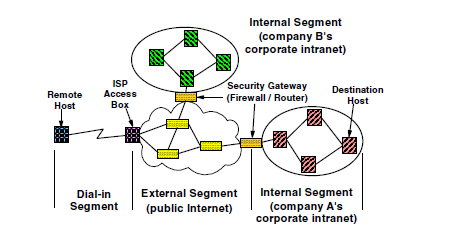
\includegraphics[scale=1]{TypicalElementsEnd-To-End-Path.png}
\end{figure}

%---------------------------------------------------------------
\newpage
\section{VPN Traffic Through Firewall}

\begin{figure}[hbtp]
\centering
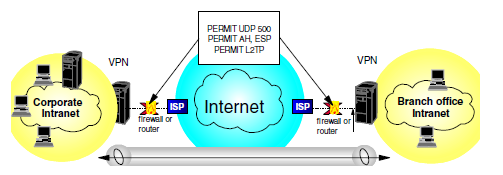
\includegraphics[scale=1]{VPN-Traffic-Through-FireWall.png}
\end{figure}


%---------------------------------------------------------------
\newpage
\section{Branch Office VPN}

\begin{figure}[hbtp]
\centering
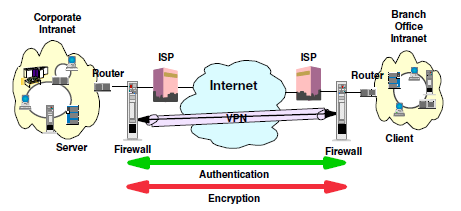
\includegraphics[scale=1]{Branch Office VPN.png}
\end{figure}

%---------------------------------------------------------------
\newpage
\section{Extranet VPN}

\begin{figure}[hbtp]
\centering
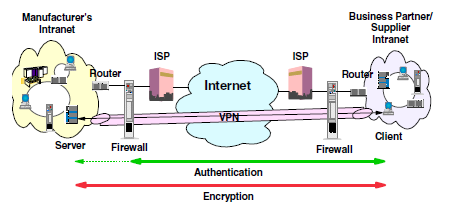
\includegraphics[scale=1]{Extranet-VPN.png}
\end{figure}


%---------------------------------------------------------------
\newpage
\section{Remote Access VPN}

\begin{figure}[hbtp]
\centering
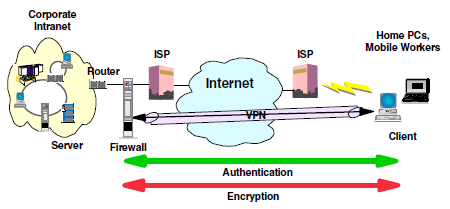
\includegraphics[scale=1]{Remote Access VPN.png}
\end{figure}

%---------------------------------------------------------------
\newpage
\section{Security Solutions In the TCP/IP Layers}

\begin{figure}[hbtp]
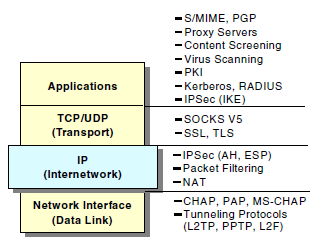
\includegraphics[scale=1]{Security Solutions In the TCP IP Layers.png}
\end{figure}

%---------------------------------------------------------------
\newpage
\section{L2TP Scenario}

\begin{figure}[hbtp]
\centering
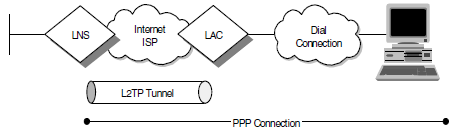
\includegraphics[scale=1]{L2TP_Scenario.png}
\end{figure}

%---------------------------------------------------------------
\newpage
\section{L2TP Compulsory}

\begin{figure}[hbtp]
\centering
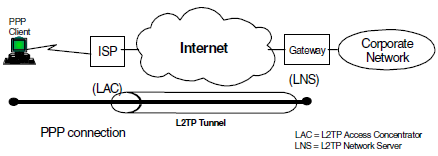
\includegraphics[scale=1]{L2TPCompulsory.png}
\end{figure}

%---------------------------------------------------------------
\newpage
\section{L2TP Voluntary}

\begin{figure}[hbtp]
\centering
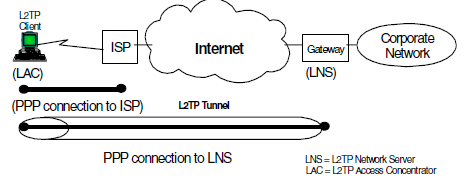
\includegraphics[scale=1]{L2TPVoluntary.png}
\end{figure}

















\end{document}